\chapter{Resultados Parciais}
\label{cap:04}

Baseado no cronograma porposto, esta sessão tem como objetivo discutir os resultados parciais de cada nó do diagrama anteriormente
apresentado.

\section{Desenvolvimento}

Idealizando o projeto como um todo e utilizando a ferramenta Obsidian\footnote{Disponível em: https://obsidian.md/} como notas, foi possível
compreender melhor o projeto e planejar novas implementações no NITE. Com a ideia geral do editor finalizada, como deverá se comportar e a forma
como os comandos do editor irão funcionar (além de seus dois modos) entre outras funcionalidades descritas, a criação de protótipos se fez necessário
para a complementação do projeto final.

\subsection{Interface Inicial}

Diferente do editor NANO, que ao ser chamado sozinho\footnote{Quando nenhum arquivo é aberto ou criado ao ser chamado via terminal}
abre diretamente na tela de edição, com informações de versão no topo e comandos abaixo, foi idealizado criar uma ``tela inicial'' para o NITE,
como as vistas no Vim e seus derivados, a diferença é que os mesmos são altamente personalizáveis, funcionalidade que não será implementada.

\FloatBarrier
\begin{figure}[!htbp]
    \centering
    \caption{Tela inicial do NITE}
    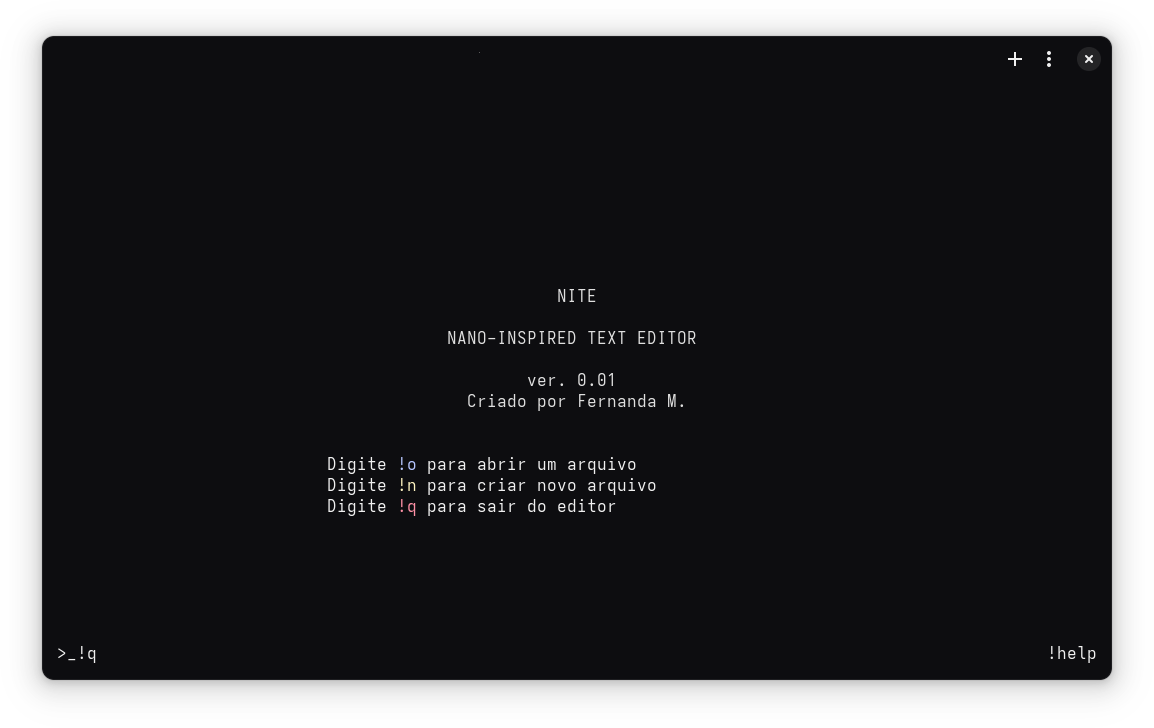
\includegraphics[scale=0.3]{imagens/NITE.png}
    \\\textbf{Fonte: O autor} \label{fig:NITE}
\end{figure}
\FloatBarrier

Como mostra a Figura~\ref{fig:NITE}, as ideias anteriormente descritas no Obsidian ganharam forma, obtendo inicialmente esta tela de apresentação,
onde o usuário tem acesso a comandos rápidos (e essenciais) para o funcionamento de qualquer eitor: criar ou abrir arquivo.
Ainda, além do comando de saída do editor, o protótipo possuí o comando de ajuda, que deverá abrir um guia de comandos que serão
implementados para navegação e funcionamento do NITE, além de explicar os modos leitura e edição.

\subsection{Criação e abertura de arquivo}

Passando para o proximo nó do diagrama e essencial para funcionamento de qualquer editor de texto, o próximo passo foi a implementação
de criação de arquivo. Com um ``\textit{extends}'', a implementação dessa funcionalidade também conta com a edição de arquivo.

Ao criar um arquivo no NITE, o mesmo pergunta o nome que o usuário pretende dar ao \textit{file} (posteriormente poderá ser editado),
podendo ou não conter uma extensão válida. As extenções aceitas e não aceitas podem ser vistas na tabela abaixo:

\begin{table}[h]
    \centering
    \caption{Extensões de arquivos aceitos e bloqueados pelo editor NITE}
    \renewcommand{\arraystretch}{1.3}
    \setlength{\tabcolsep}{8pt}
    \begin{tabular}{@{}p{3.5cm}p{5.2cm}p{5.2cm}@{}}
        \toprule
        \textbf{Categoria} &
        \textbf{Extensões válidas} &
        \textbf{Extensões não válidas} \\
        \midrule
        \textbf{Texto plano} &
        .txt, .md, .csv, .log &
        – \\

        \textbf{Código-fonte} &
        Arquivos de texto contendo código de linguagens de programação
        (ex.: .c, .cpp, .java, .py, .js, .html, .css, .json, .xml, etc.) &
        – \\

        \textbf{Configurações} &
        .ini, .conf, .properties, .toml &
        – \\

        \textbf{Executáveis / Binários} &
        – &
        .exe, .dll, .so, .bin, .out, .app \\

        \textbf{Mídia (imagens / áudio / vídeo)} &
        – &
        .png, .jpg, .jpeg, .gif, .bmp, .mp3, .mp4, .wav \\

        \textbf{Compactados} &
        – &
        .zip, .rar, .tar, .gz, .7z \\

        \textbf{Documentos binários} &
        – &
        .doc, .docx, .pptx, .xlsx, .pdf \\

        \textbf{Imagens de disco} &
        – &
        .iso, .img \\

        \textbf{Scripts executáveis*} &
        – &
        .sh, .bat, .ps1, .cmd \\
        \bottomrule
    \end{tabular}

    \footnotesize\\[0.5em]
    *Podem ser aceitos futuramente.
\end{table}

Caso uma das extensão não aceitas for chamada, o editor irá mostrar um erro e solicitar que o usuário crie um arquivo válido. Em caso do usuário
não fornecer uma extensão, o editor continuará o processo normalmente passando para a página de edição.

Inicialmente, o protótipo conta com as seguintes informações no topo do arquivo: Nome do arquivo sendo editado, F1 para salvar e F2 para sair
do editor. Ambas as funcionalidades abrirão uma nova janela, que confirma a saída ou o salvamento do arquivo.

\FloatBarrier
\begin{figure}[!htbp]
    \centering
    \caption{NITE confirmando o salvamento de arquivo}
    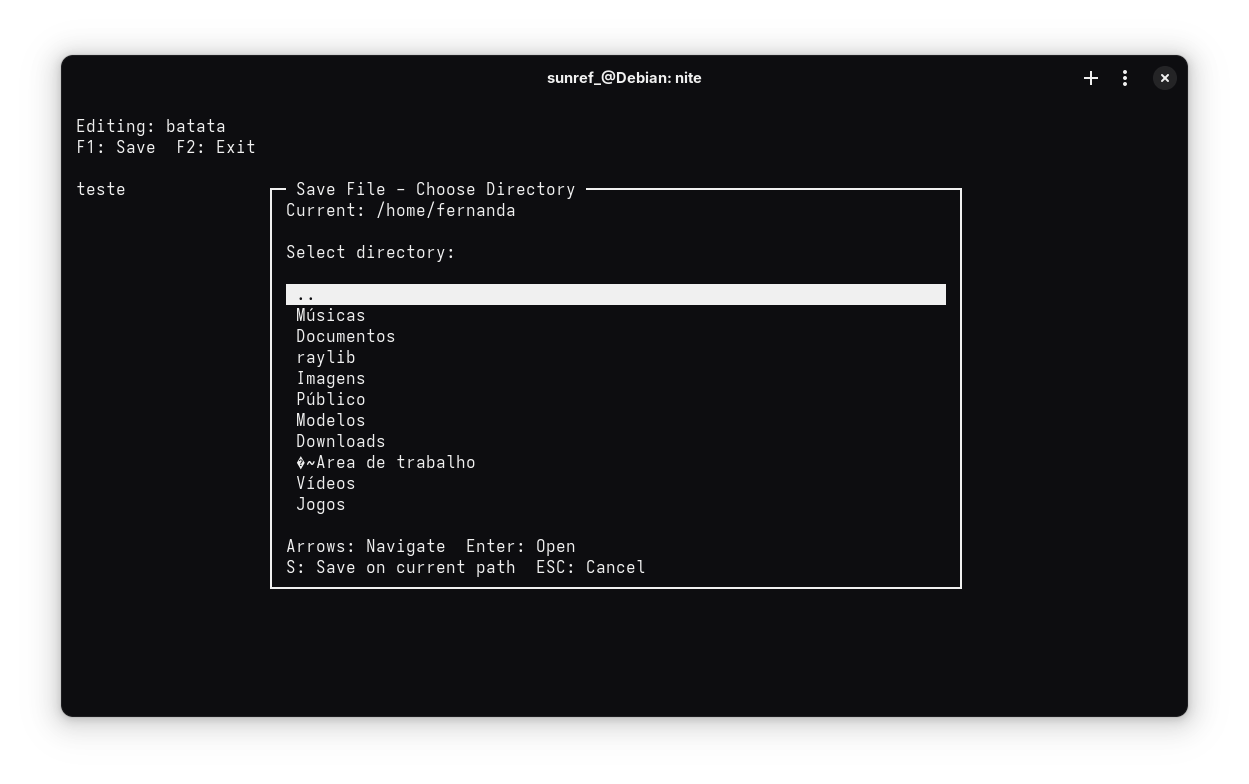
\includegraphics[scale=0.3]{imagens/ConfirmSave.png}
    \\\textbf{Fonte: O autor} \label{fig:ConfirmSave}
\end{figure}
\FloatBarrier

Caso o usuário resolva sair do editor sem salvar o arquivo, uma mensagem é exibida no terminal após a saida. Caso o arquivo foi salvo, após a saida
do editor, outra mensagem é exibida.

\section{Repositório do Github}

O código base do editor e este documento se encontram disponíveis no link do Github: \url{https://github.com/Sunref/nite}

\section{Cronograma do Trabalho}

Segue abaixo o cronograma de trabalho das atividades realizadas.

\FloatBarrier
\begin{figure*}[!htbp]
	\centering
	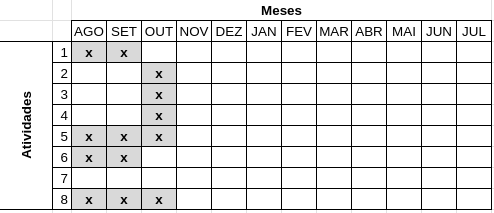
\includegraphics[scale=0.4]{imagens/cronograma.png}
\end{figure*}
\FloatBarrier

\begin{enumerate}
	\item Atividade 01: Implementação do protótipo inicial;
	\item Atividade 02: Criação e abertura de arquivos;
	\item Atividade 03: Edição e e Salvamento de arquivo;
	\item Atividade 04: Suporte a multiplos arquivos;
	\item Atividade 05: Atalhos de teclado;
	\item Atividade 06: Ajustes visuais e de interface;
	\item Atividade 07: Destaque de sintaxe;
	\item Atividade 08: Buscar outras funcionalodades para implementação.
\end{enumerate}